\begin{activity} \label{A:7.2.1}  
  Warfarin is an anticoagulant that prevents blood clotting; often it is prescribed to stroke victims in order  to help ensure blood flow. The level of warfarin has to reach a certain concentration in the blood in order to be effective. 

Suppose warfarin is taken by a particular patient in a 5 mg dose each day. The drug is absorbed by the body and some is excreted from the system between doses. Assume that at the end of a 24 hour period, 8\% of the drug remains in the body. Let $Q(n)$ be the amount (in mg) of warfarin in the body before the $(n+1)$st dose of the drug is administered.

\ba
\item Explain why $Q(1) = 5 \times 0.08$ mg.

\item Explain why $Q(2) = (5+Q(1)) \times 0.08$ mg. Then show that 
\[Q(2) = (5 \times 0.08)\left(1+0.08\right) \text{ mg}.\]

\item Explain why $Q(3) = (5+Q(2)) \times 0.08$ mg. Then show that
\[Q(3) = (5 \times 0.08)\left(1+0.08+0.08^2\right) \text{ mg}.\]

\item Explain why $Q(4) = (5+Q(3)) \times 0.08$ mg. Then show that
\[Q(4) = (5 \times 0.08)\left(1+0.08+0.08^2+0.08^3\right) \text{ mg}.\]

\item There is a pattern that you should see emerging. Use this pattern to find a formula for $Q(n)$, where $n$ is an arbitrary positive integer.

\item Complete Table \ref{T:8.2_Warfarin} with values of $Q(n)$ for the provided $n$-values (reporting $Q(n)$ to 10 decimal places). What appears to be happening to the sequence $Q(n)$ as $n $ increases?
\begin{table}[ht]
\begin{center}
\renewcommand{\arraystretch}{1.5}
\begin{tabular}{c|c}
$Q(1)$   & $0.40$ \\
$Q(2)$   & \\
$Q(3)$   &  \\
$Q(4)$   &  \\
$Q(5)$   &  \\
$Q(6)$   &  \\
$Q(7)$   &  \\
$Q(8)$   &  \\
$Q(9)$   &  \\
$Q(10)$  &  \\
\end{tabular}
\caption{Values of $Q(n)$ for selected values of $n$}
\label{T:8.2_Warfarin}
\end{center}
\end{table}

%\begin{itemize}
%\item After the first dose is administered, the body will absorb the drug and retain 8\% of the dose. So
%\[Q(1) = 5 \times 0.08 \text{ mg}.\]
%\item After the second dose is administered, the body will absorb the drug and retain 8\% of the dose, plus what remained in the body after the second dose. So
%\[Q(2) = 5 \times 0.08 + \left(0.08 \times 5\right) \times 0.08 = (5 \times 0.08)\left(1+0.08\right) \text{ mg}.\]
%\item After the third dose is administered, the body will absorb the drug and retain 8\% of the dose, plus what remained in the body after the third dose. So
%\[Q(3) = 5 \times 0.08 + \left(0.08 \times 5\right) \left(1+0.08\right)\times 0.08 = (5 \times 0.08)\left(1+0.08+0.08^2\right) \text{ mg}.\]
%\item After the fourth dose is administered, the body will absorb the drug and retain 8\% of the dose, plus what remained in the body after the fourth dose. So
%\[Q(4) = 5 \times 0.08 + \left(0.08 \times 5\right) \left(1+0.08+0.08^2\right)\times 0.08 = (5 \times 0.08)\left(1+0.08+0.08^2+0.08^3\right) \text{ mg}.\]
%\end{itemize}


%A pattern seems to be emerging. It appears that after the $n$th dose is administered, the body will absorb the drug and retain 8\% of the dose, plus what remained in the body after the $n$th dose and so
%\begin{equation} \label{eq:8.2_part_sum}
%Q(n)=(5 \times 0.08)\left(1+0.08+0.08^2+0.08^3+ \cdots + 0.08^{n-1}\right) \text{ mg}.
%\end{equation}

%*** begin comment ***

%Table \ref{T:8.2_Warfarin} gives the values of $Q(n)$ for a few selected values (to 10 decimal places) of $n$:
%\begin{table}[ht]
%\begin{center}
%\renewcommand{\arraystretch}{1.5}
%\begin{tabular}{c|c}
%$Q(1)$   & $0.40$ \\
%$Q(2)$   & $0.432$ \\
%$Q(3)$   & $0.43456$ \\
%$Q(4)$   & $0.4347648$ \\
%$Q(5)$   & $0.434781184$ \\
%$Q(6)$   & $0.4347824948$ \\
%$Q(7)$   & $0.4347825996$ \\
%$Q(8)$   & $0.4347826080$ \\
%$Q(9)$   & $0.4347826088$ \\
%$Q(10)$  & $0.4347826088$ \\
%\end{tabular}
%\caption{Values of $Q(n)$ for selected values of $n$}
%\label{T:8.2_Warfarin_Sol}
%\end{center}
%\end{table}
%We can plot the data points $(n,Q(n))$ and visualize the long-term behavior as shown in Figure \ref{F:8.2.Warfarin}

%\begin{figure}[h]
%\begin{center}
%\resizebox{!}{1.5in}{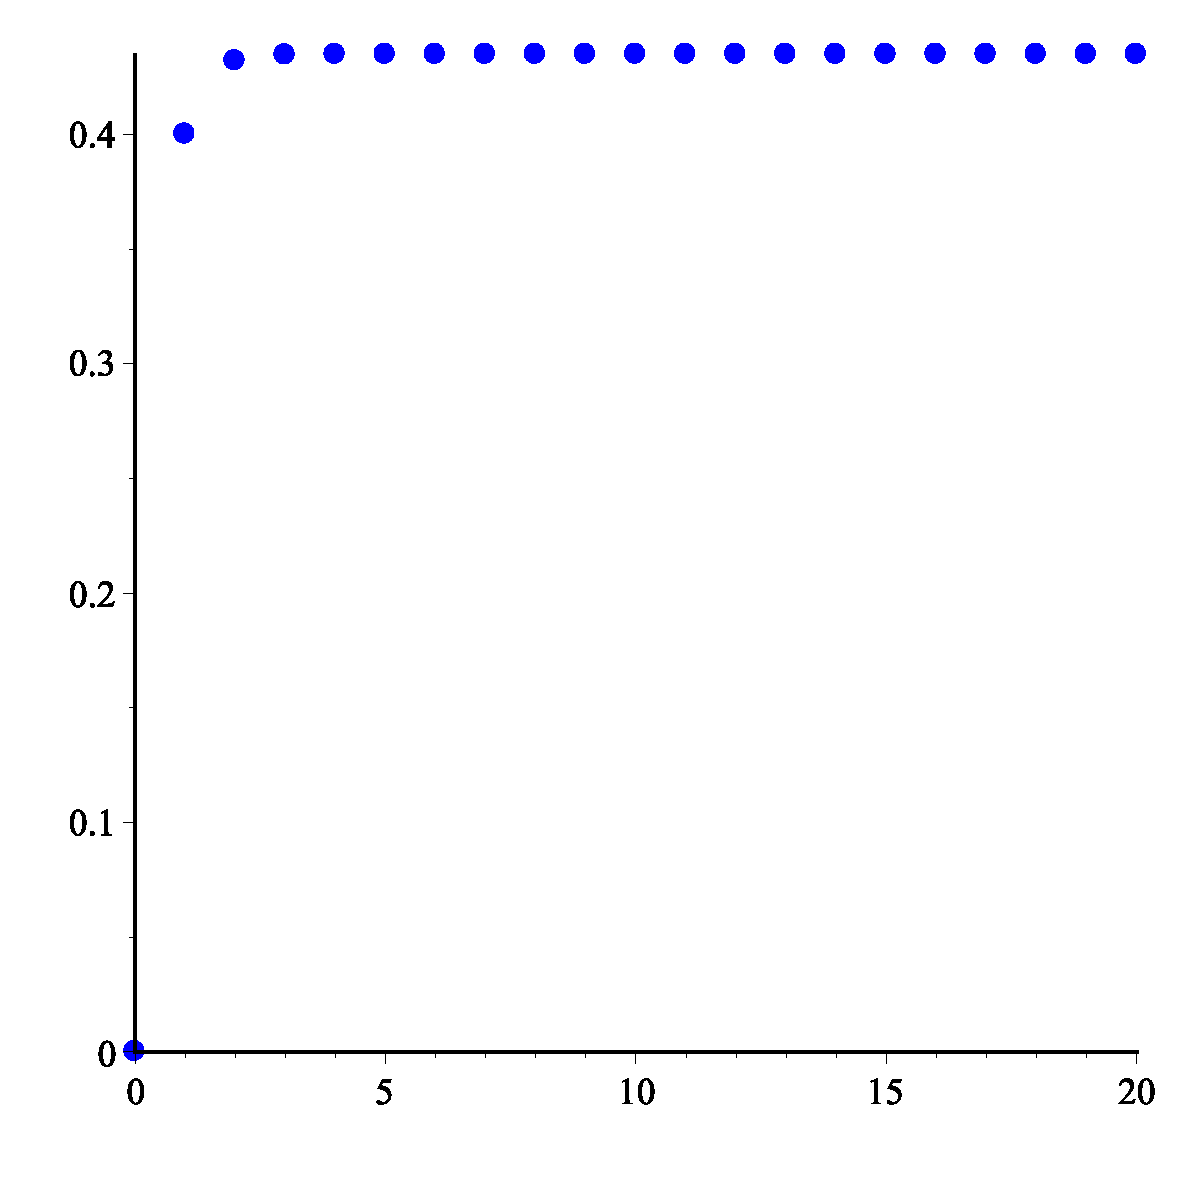
\includegraphics{figures/8_2_Warfarin.eps}}
%\caption{The points $(n, Q(n))$ for $n$ from 1 to 20}
%\label{F:8.2.Warfarin}
%\end{center}
%\end{figure}

%The data and the graph appears to indicate there is a long-term level of Warfarin that remains in the blood, or a limit to the sequence of values $Q(n)$ as $n$ goes to infinity. The data approximates this ling-term level, but with a little more work we can find the exact level of Warfarin in the blood.

%*** end comment ****


\ea
\end{activity}


\begin{smallhint}
\ba
	\item Small hints for each of the prompts above.
\ea
\end{smallhint}
\begin{bighint}
\ba
	\item Big hints for each of the prompts above.
\ea
\end{bighint}
\begin{activitySolution}
\ba
	\item Solutions for each of the prompts above.
\ea
\end{activitySolution}
\aftera